\documentclass{beamer}

% german content
% \usepackage[ngerman]{babel}

% images
\usepackage{graphicx}
\graphicspath{ {./images/} }

\title{Authentication}
\subtitle{github.com/jneidel/authentication-vortrag}
\author{Jonathan Neidel}
\date{Januar 2022}
\institute{HTW Berlin, Angewandte Informatik, Komponentenbasierte Entwicklung}
\logo{
\includegraphics[width=1cm]{logo}}

% theme + color theme
\usetheme{Szeged}
\usecolortheme{whale}
% see: https://deic-web.uab.cat/~iblanes/beamer_gallery/index.html
\setbeamerfont{caption}{size=\Tiny}

\begin{document}
\frame{\titlepage}

\begin{frame}
  \frametitle{What is authentication?}

  credentials check

  \bigskip

  Answering: Who are you?
\end{frame}

\begin{frame}
  \frametitle{Abstract process}

  user fills form with username, password
  \begin{enumerate}
    \item \begin{itemize}
      \item 401 (Authentication failed)
    \end{itemize}
    \item \begin{itemize}
      \item 200 (OK)
      \item response includes a session token
      \item set as a cookie
      \item subsequent http requests include the token
    \end{itemize}
  \end{enumerate}
\end{frame}

\begin{frame}
  \frametitle{Same-Origin-Policy}

  cookies are accessible on the domain that created them
\end{frame}

\begin{frame}
  \frametitle{What is Authorization?}

  privilege check

  \bigskip

  Answering: Are you allowed to do this?
\end{frame}

\begin{frame}
  \frametitle{Keycloak: https://www.keycloak.org}
    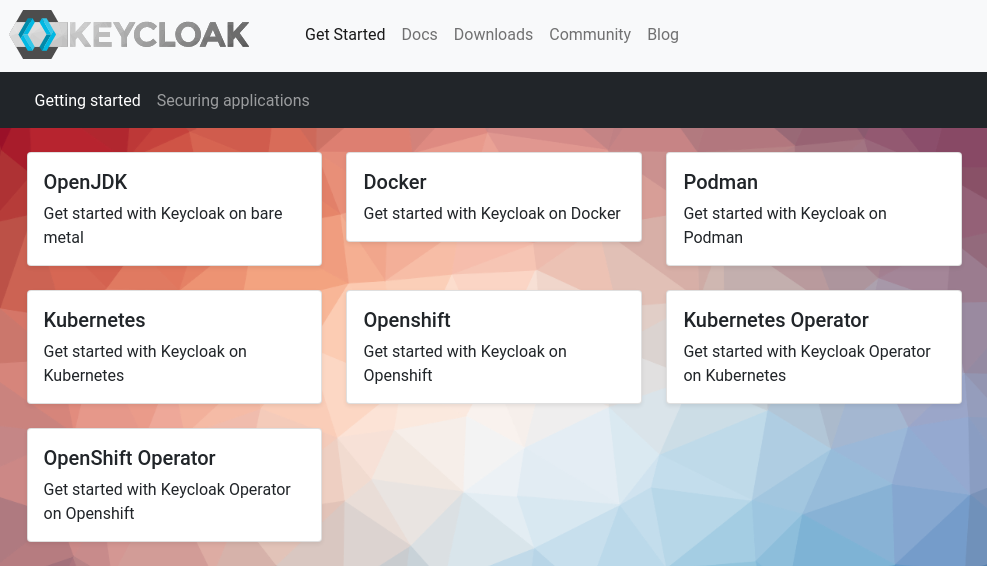
\includegraphics[width=11cm]{install}
\end{frame}

\begin{frame}
  \frametitle{References}

  \begin{itemize}
    \item What is SSO: https://auth0.com/blog/what-is-and-how-does-single-sign-on-work
    \item What is IdM: https://en.wikipedia.org/wiki/Identity\_management
    \medskip
    \item Keycloak: https://www.keycloak.org
    \item JWT: https://jwt.io
  \end{itemize}
\end{frame}

\end{document}
